\documentclass[a4paper]{standalone}
\usepackage[a4paper,margin=25mm]{geometry}
\usepackage{graphicx,subcaption}
\usepackage{amsmath,amsfonts}
\usepackage{qtree}
\usepackage{tikz}
\usepackage{varwidth}

\newcommand{\rvec}[1]{\accentset{\leftarrow}{#1}}
\newcommand{\Bb}[1]{%
  \expandafter\def\csname#1#1\endcsname%
  {\ensuremath{\mathbb #1}}}
\Bb X\Bb S\Bb V\Bb Z
\newcommand{\up}{\!\uparrow}
\newcommand{\dn}{\downarrow\!}
\newcommand{\ui}{\underline{\iota}}
\newcommand{\ut}{\underline{\tau}}
\newcommand{\ur}{\underline{r}}
\newcommand{\vr}{\vec{r}}
\newcommand{\uvr}{\underline{\vr}}
\newcommand{\tm}{\tau^{-}}
\newcommand{\vs}{\vec{s}}
\newcommand{\uvs}{\underline{\vs}}
\newcommand{\vx}{\vec{x}}
\newcommand{\uvx}{\underline{\vx}}
\newcommand{\ux}{\underline{x}}
\newcommand{\us}{\underline{s}}

\begin{document}
\begin{figure}[hbt]
\centering
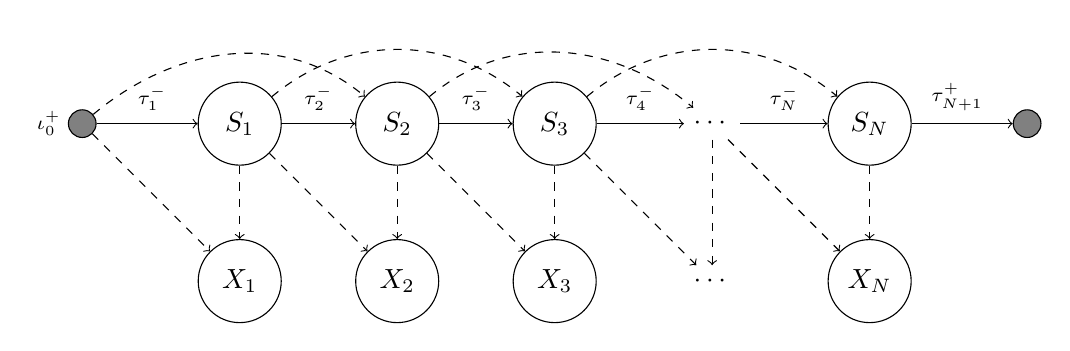
\begin{tikzpicture}[cnode/.style={draw,circle,minimum size=3em,inner sep=3pt}, onode/.style={fill=black!50, draw,circle,minimum size=1em}]
    \node (0i) at (-0.7,0) [right] {$\stackrel{\iota_0^+}{}$};
    \node[onode] (0) at (0,0) {};
    \node[cnode] (1) at (2,0) {$S_1$};
    \node[cnode] (1x) at (2,-2) {$X_1$};
    \node[cnode] (2) at (4, 0)  {$S_2$};
    \node[cnode] (2x) at (4, -2)  {$X_2$};
    \node[cnode] (3) at (6, 0)  {$S_3$};
    \node[cnode] (3x) at (6, -2)  {$X_3$};
    \node (t) at (8, 0) {$\cdots$};
    \node (tx) at (8, -2) {$\cdots$};
    \node[cnode] (N) at (10, 0)  {$S_N$};
    \node[cnode] (Nx) at (10, -2)  {$X_N$};
    \node[onode] (tt) at (12, 0) {};

    \draw[->] (0) edge node [pos=0.55, above] {$\stackrel{\tm_1}{}$}  (1) ;
    \draw[->] (1) edge node [pos=0.5, above] {$\stackrel{\tm_2}{}$}  (2) ;
    \draw[->] (2) edge node [pos=0.5, above] {$\stackrel{\tm_3}{}$}  (3) ;
    \draw[->] (3) edge node [pos=0.5, above] {$\stackrel{\tm_4}{}$}  (t) ;
    \draw[->] (t) edge node [pos=0.5, above] {$\stackrel{\tm_N}{}$}  (N) ;
    \draw[->] (N) edge node [pos=0.45, above] {$\stackrel{\tau^+_{N+1}}{}$} (tt) ;

   \begin{scope}[dashed]
    \draw[->] (0) to[out=40,in=140] (2) ;
    \draw[->] (1) to[out=40,in=140] (3) ;
    \draw[->] (2) to[out=40,in=140] (t) ;
    \draw[->] (3) to[out=40,in=140] (N) ;
   \end{scope}

   \begin{scope}[dashed]
    \draw[->] (0) to (1x) ;
    \draw[->] (1) to (1x) ;
    \draw[->] (1) to (2x) ;
    \draw[->] (2) to (2x) ;
    \draw[->] (2) to (3x) ;
    \draw[->] (3) to (3x) ;
    \draw[->] (3) to (tx) ;
    \draw[->] (t) to (tx) ;
    \draw[->] (t) to (Nx) ;
    \draw[->] (N) to (Nx) ;
   \end{scope}

\end{tikzpicture}
\end{figure}
\end{document}